%% Creator: Inkscape 1.2.2 (b0a8486541, 2022-12-01), www.inkscape.org
%% PDF/EPS/PS + LaTeX output extension by Johan Engelen, 2010
%% Accompanies image file 'CAPA_FINAL-modelo_latex.pdf' (pdf, eps, ps)
%%
%% To include the image in your LaTeX document, write
%%   \input{<filename>.pdf_tex}
%%  instead of
%%   \includegraphics{<filename>.pdf}
%% To scale the image, write
%%   \def\svgwidth{<desired width>}
%%   \input{<filename>.pdf_tex}
%%  instead of
%%   \includegraphics[width=<desired width>]{<filename>.pdf}
%%
%% Images with a different path to the parent latex file can
%% be accessed with the `import' package (which may need to be
%% installed) using
%%   \usepackage{import}
%% in the preamble, and then including the image with
%%   \import{<path to file>}{<filename>.pdf_tex}
%% Alternatively, one can specify
%%   \graphicspath{{<path to file>/}}
%% 
%% For more information, please see info/svg-inkscape on CTAN:
%%   http://tug.ctan.org/tex-archive/info/svg-inkscape
%%
\begingroup%
  \makeatletter%
  \providecommand\color[2][]{%
    \errmessage{(Inkscape) Color is used for the text in Inkscape, but the package 'color.sty' is not loaded}%
    \renewcommand\color[2][]{}%
  }%
  \providecommand\transparent[1]{%
    \errmessage{(Inkscape) Transparency is used (non-zero) for the text in Inkscape, but the package 'transparent.sty' is not loaded}%
    \renewcommand\transparent[1]{}%
  }%
  \providecommand\rotatebox[2]{#2}%
  \providecommand*\fsize{\dimexpr\f@size pt\relax}%
  \providecommand*\lineheight[1]{\fontsize{\fsize}{#1\fsize}\selectfont}%
  \ifx\svgwidth\undefined%
    \setlength{\unitlength}{1281.25982666bp}%
    \ifx\svgscale\undefined%
      \relax%
    \else%
      \setlength{\unitlength}{\unitlength * \real{\svgscale}}%
    \fi%
  \else%
    \setlength{\unitlength}{\svgwidth}%
  \fi%
  \global\let\svgwidth\undefined%
  \global\let\svgscale\undefined%
  \makeatother%
  \begin{picture}(1,0.70132751)%
    \lineheight{1}%
    \setlength\tabcolsep{0pt}%
    %\put(0,0){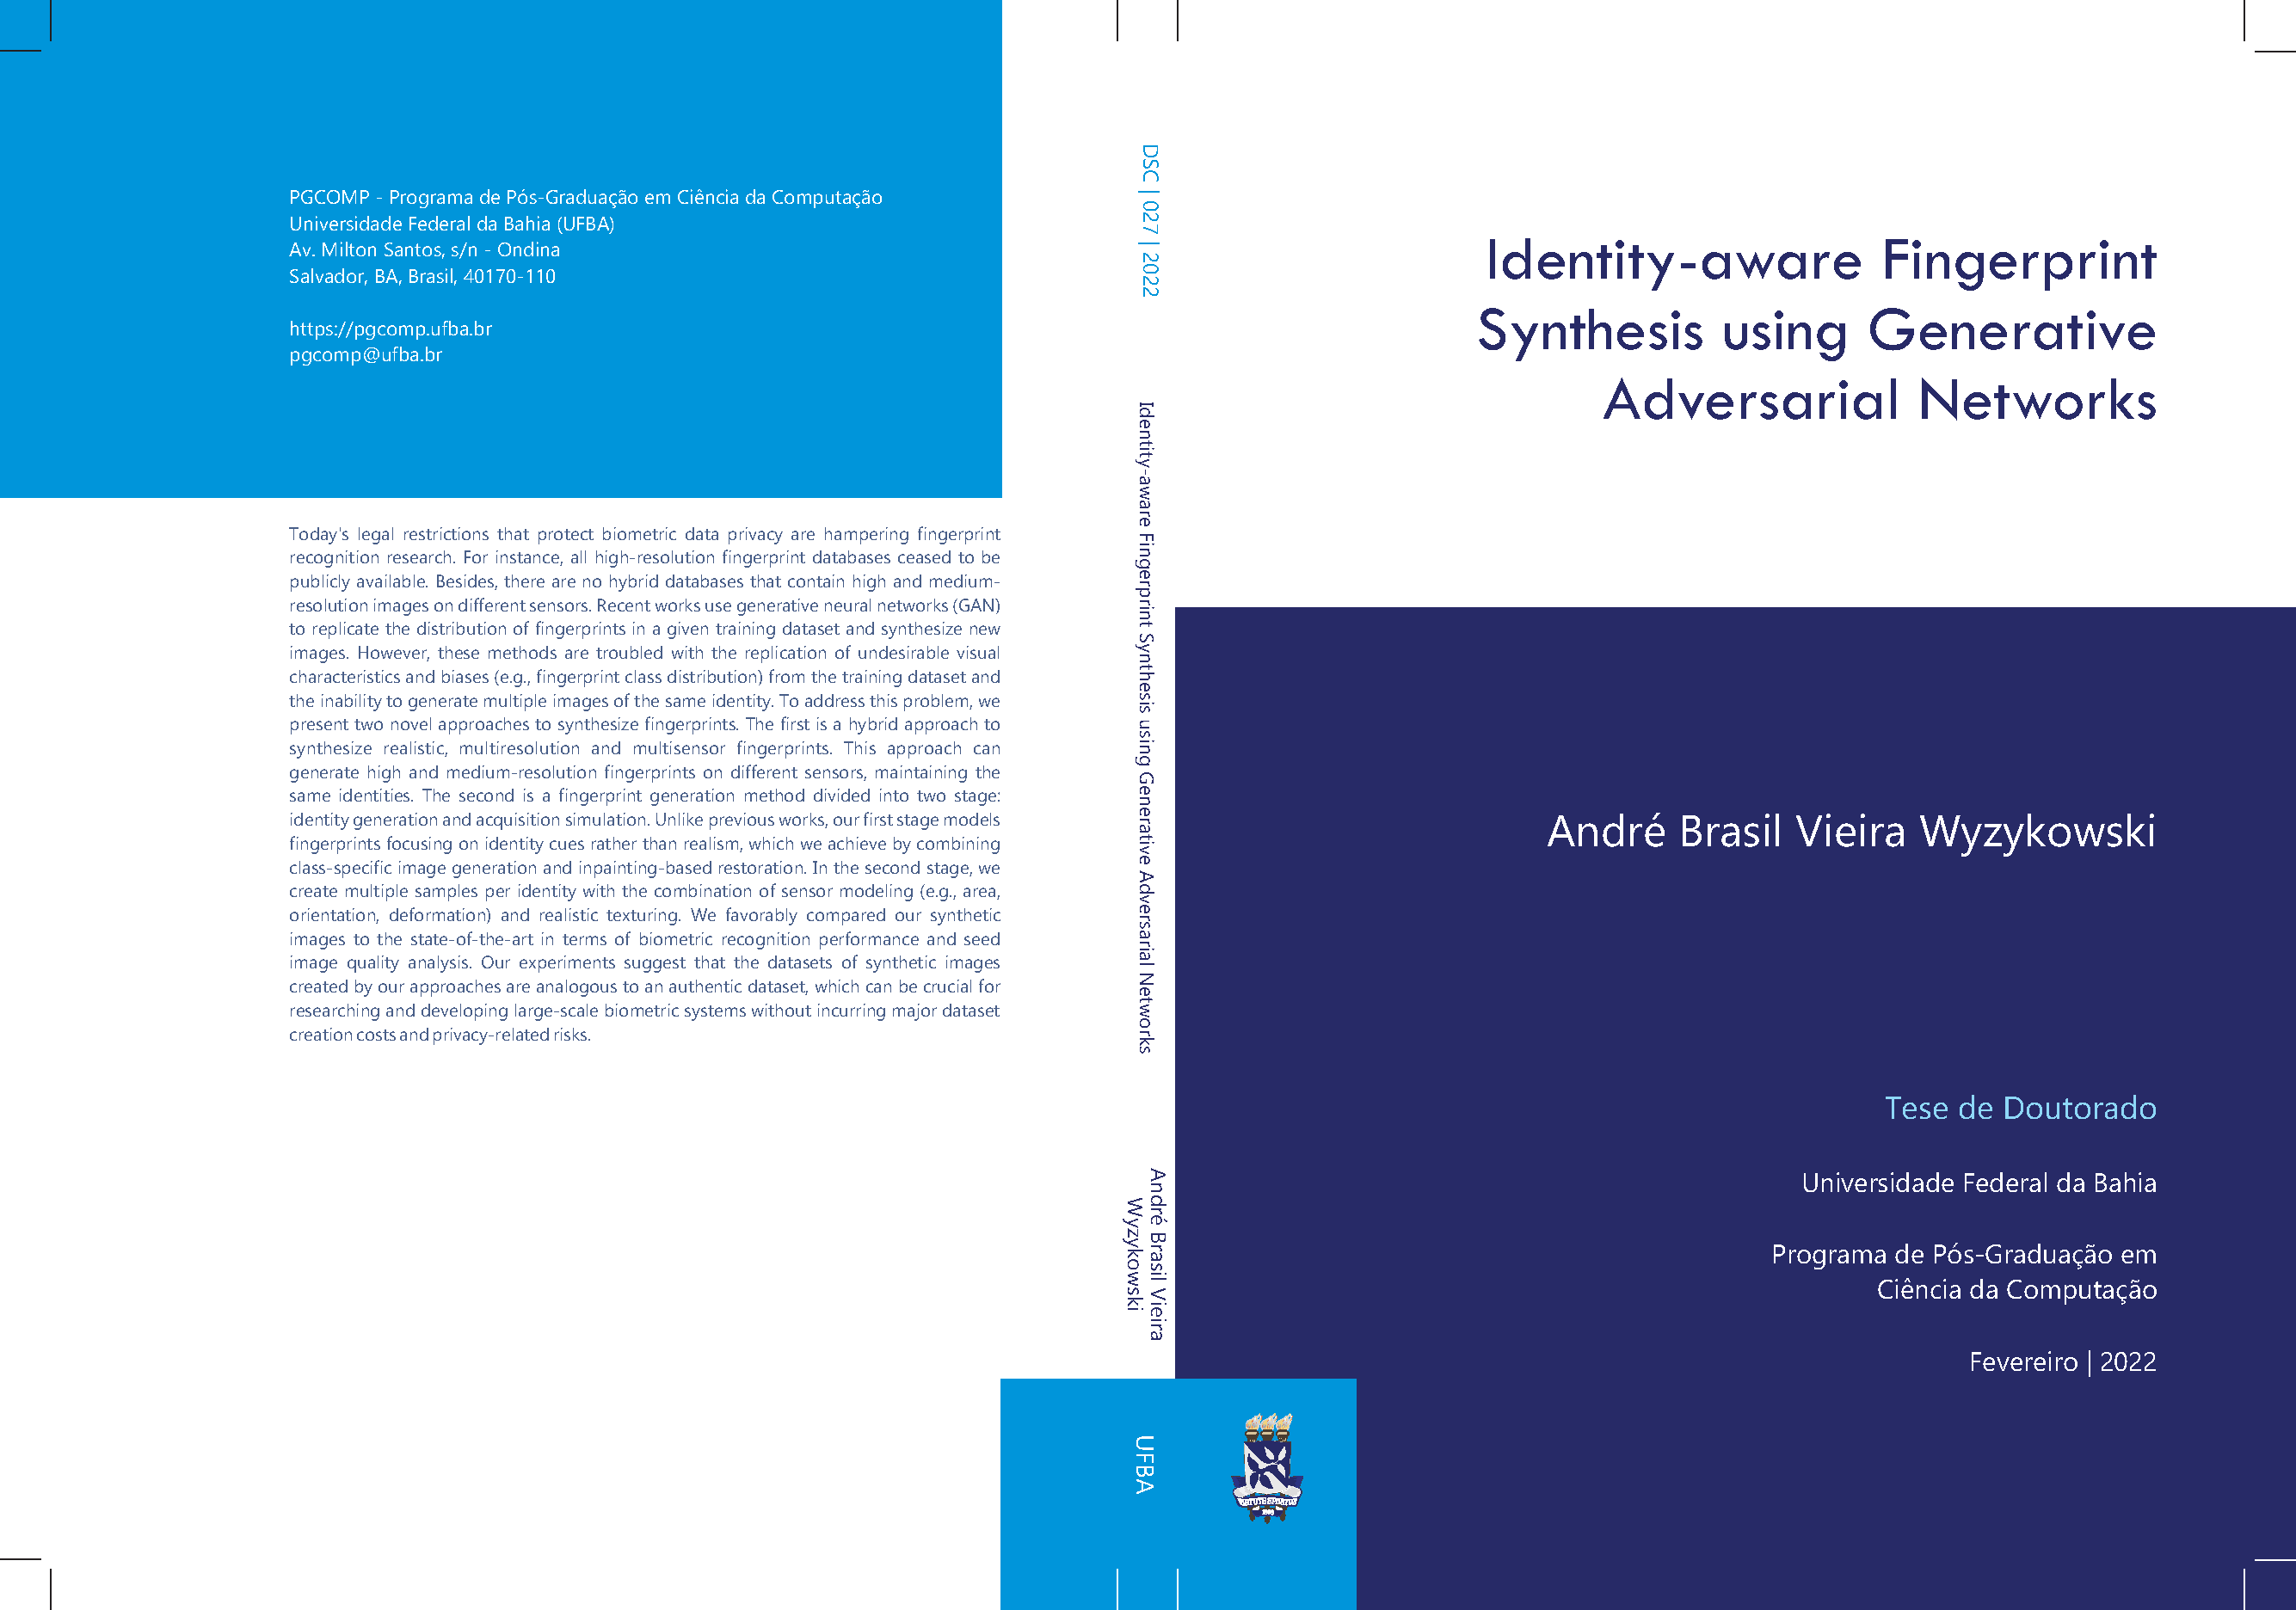
\includegraphics[width=\unitlength,page=1]{CAPA_FINAL-modelo.pdf}}%
    \put(0,0){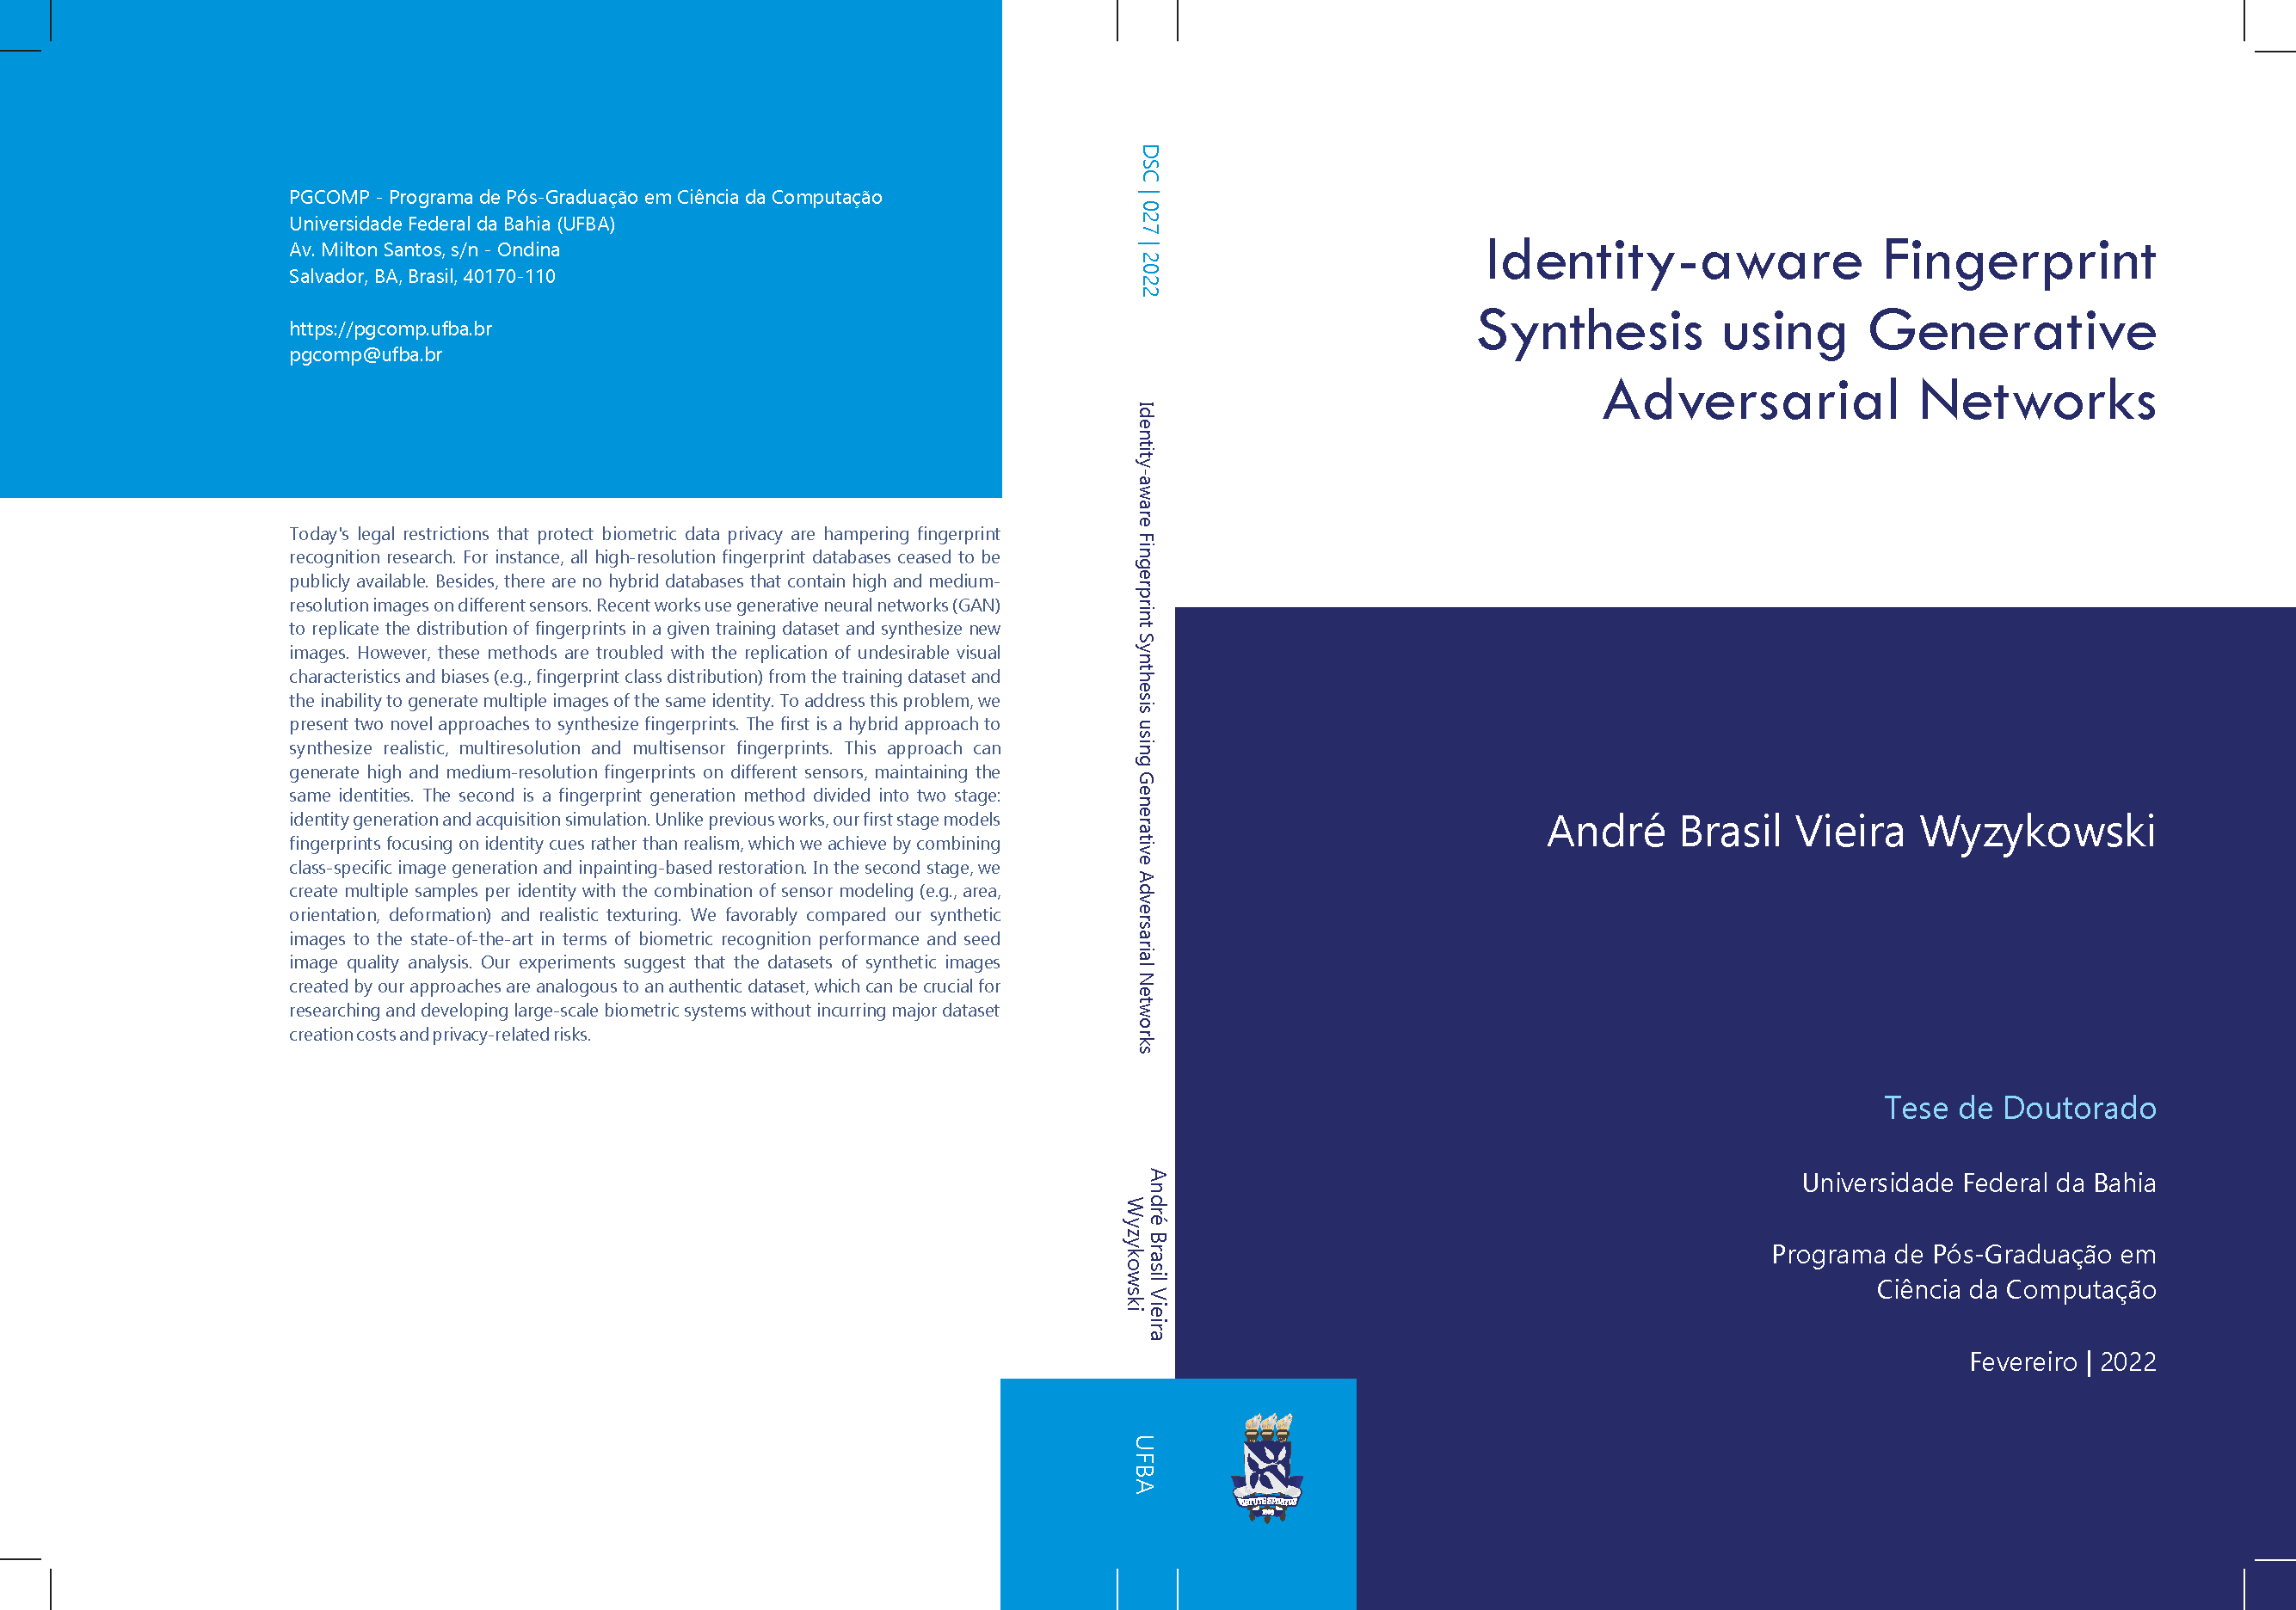
\includegraphics[width=\unitlength,page=1]{CAPA_FINAL-modelo_croped_cmyk.pdf}}
    \put(0.59070796,0.57991487){\color[rgb]{0,0,0}\makebox(0,0)[lt]{\lineheight{1.25}\smash{\begin{tabular}[t]{R{0.73\textwidth}}\fontsize{36.15}{39.25}\TwCenMT{Identity-aware Fingerprint Synthesis using Generative Adversarial Networks}\end{tabular}}}}%
    \put(0.59070796,0.33259119){\color[rgb]{0,0,0}\makebox(0,0)[lt]{\lineheight{1.25}\smash{\begin{tabular}[t]{R{0.73\textwidth}}\fontsize{25.13}{1.25}\ebrima{André Brasil Vieira Wyzykowski}\end{tabular}}}}%
    \put(0.12603759,0.46617283){\color[rgb]{0,0,0}\makebox(0,0)[lt]{\lineheight{1.25}\smash{\begin{tabular}[t]{J{0.65\textwidth}}\fontsize{10}{13.355}\ebrima{Today's legal restrictions that protect biometric data privacy are hampering fingerprint recognition research. For instance, all high-resolution fingerprint databases ceased to be publicly available. Besides, there are no hybrid databases that contain high and medium-resolution images on different sensors. Recent works use generative neural networks (GAN) to replicate the distribution of fingerprints in a given training dataset and synthesize new images. However, these methods are troubled with the replication of undesirable visual characteristics and biases (e.g., fingerprint class distribution) from the training dataset and the inability to generate multiple images of the same identity. To address this problem, we present two novel approaches to synthesize fingerprints. The first is a hybrid approach to synthesize realistic, multiresolution and multisensor fingerprints. This approach can generate high and medium-resolution fingerprints on different sensors, maintaining the same identities. The second is a fingerprint generation method divided into two stage: identity generation and acquisition simulation. Unlike previous works, our first stage models fingerprints focusing on identity cues rather than realism, which we achieve by combining class-specific image generation and inpainting-based restoration. In the second stage, we create multiple samples per identity with the combination of sensor modeling (e.g., area, orientation, deformation) and realistic texturing. We favorably compared our synthetic images to the state-of-the-art in terms of biometric recognition performance and seed image quality analysis. Our experiments suggest that the datasets of synthetic images created by our approaches are analogous to an authentic dataset, which can be crucial for researching and developing large-scale biometric systems without incurring major dataset creation costs and privacy-related risks.}\end{tabular}}}}%
    \put(0.12603759,0.6124423){\color[rgb]{0,0,0}\makebox(0,0)[lt]{\lineheight{1.466}\smash{\fontsize{11.054}{1.25}\begin{tabular}[t]{l}\ebrima{PGCOMP - Programa de Pós-Graduação em Ciência da Computação}\\\ebrima{Universidade Federal da Bahia (UFBA)}\\\ebrima{Av. Milton Santos, s/n - Ondina}\\\ebrima{Salvador, BA, Brasil, 40170-110}\\\\\ebrima{https://pgcomp.ufba.br}\\\ebrima{pgcomp@ufba.br}\end{tabular}}}}%
    \put(0.4950728,0.07637041){\color[rgb]{0,0,0}\rotatebox{-90}{\makebox(0,0)[lt]{\lineheight{1.25}\smash{\begin{tabular}[t]{l}\fontsize{14}{1.25}\ebrima{UFBA}\end{tabular}}}}}%
    \put(0.59070796,0.21391464){\color[rgb]{0,0,0}\makebox(0,0)[lt]{\lineheight{1.25}\smash{\begin{tabular}[t]{>{\raggedleft}p{0.73\textwidth}}\fontsize{18}{1.25}\ebrima{Tese de Doutorado}\end{tabular}}}}%
    \put(0.59070796,0.18218165){\color[rgb]{0,0,0}\makebox(0,0)[lt]{\lineheight{2}\smash{\fontsize{15}{1.25}\begin{tabular}[t]{R{0.73\textwidth}}\ebrima{Universidade Federal da Bahia}\\\\\ebrima{Programa de Pós-Graduação em}\\\ebrima{Ciência da Computação}\\\\\ebrima{Fevereiro | 2022}\end{tabular}}}}%
    \put(0.49782899,0.63889314){\color[rgb]{0,0,0}\rotatebox{-90}{\makebox(0,0)[lt]{\lineheight{1.25}\smash{\fontsize{12}{1.25}\begin{tabular}[t]{l}\ebrima{DSC | 027 | 2022}\end{tabular}}}}}%
    \put(0.49644488,0.5493505){\color[rgb]{0,0,0}\rotatebox{-90}{\makebox(0,0)[lt]{\lineheight{1.25}\smash{\fontsize{11.054}{1.25}\begin{tabular}[t]{C{0.69\textwidth}}\ebrima{Identity-aware Fingerprint Synthesis using Generative Adversarial Networks}\end{tabular}}}}}%
    \put(0.50110506,0.20886039){\color[rgb]{0,0,0}\rotatebox{-90}{\makebox(0,0)[lt]{\lineheight{1.25}\smash{\begin{tabular}[t]{C{0.225\textwidth}}\fontsize{12}{13.39}\ebrima{André Brasil Vieira Wyzykowski}\end{tabular}}}}}%
  \end{picture}%
\endgroup%
